\documentclass[a4paper,14pt, unknownkeysallowed]{extreport}

\usepackage{cmap} % Улучшенный поиск русских слов в полученном pdf-файле
\usepackage[T2A]{fontenc} % Поддержка русских букв
\usepackage[utf8]{inputenc} % Кодировка utf8
\usepackage[english,russian]{babel} % Языки: русский, английский
\usepackage{enumitem}


\usepackage{threeparttable}

\usepackage[14pt]{extsizes}

\usepackage{caption}
\captionsetup{labelsep=endash}
\captionsetup[figure]{name={Рисунок}}

% \usepackage{ctable}
% \captionsetup[table]{justification=raggedleft,singlelinecheck=off}

\usepackage{amsmath}

\usepackage{geometry}
\geometry{left=30mm}
\geometry{right=10mm}
\geometry{top=20mm}
\geometry{bottom=20mm}

\usepackage{titlesec}
\titleformat{\section}
	{\normalsize\bfseries}
	{\thesection}
	{1em}{}
\titlespacing*{\chapter}{0pt}{-30pt}{8pt}
\titlespacing*{\section}{\parindent}{*4}{*4}
\titlespacing*{\subsection}{\parindent}{*4}{*4}

\usepackage{setspace}
\onehalfspacing % Полуторный интервал

\frenchspacing
\usepackage{indentfirst} % Красная строка

\usepackage{titlesec}
\titleformat{\chapter}{\LARGE\bfseries}{\thechapter}{20pt}{\LARGE\bfseries}
\titleformat{\section}{\Large\bfseries}{\thesection}{20pt}{\Large\bfseries}

\usepackage{multirow}
\usepackage{listings}
\usepackage{xcolor}

% Для листинга кода:
\lstset{%
	language=python,   					% выбор языка для подсветки	
	basicstyle=\small\sffamily,			% размер и начертание шрифта для подсветки кода
	numbers=left,						% где поставить нумерацию строк (слева\справа)
	%numberstyle=,						% размер шрифта для номеров строк
	stepnumber=1,						% размер шага между двумя номерами строк
	numbersep=5pt,						% как далеко отстоят номера строк от подсвечиваемого кода
	frame=single,						% рисовать рамку вокруг кода
	tabsize=4,							% размер табуляции по умолчанию равен 4 пробелам
	captionpos=t,						% позиция заголовка вверху [t] или внизу [b]
	breaklines=true,					
	breakatwhitespace=true,				% переносить строки только если есть пробел
	escapeinside={\#*}{*)},				% если нужно добавить комментарии в коде
	backgroundcolor=\color{white},
}


\usepackage{pgfplots}
\usetikzlibrary{datavisualization}
\usetikzlibrary{datavisualization.formats.functions}

\usepackage{graphicx}
\newcommand{\img}[3] {
	\begin{figure}[h!]
		\center{\includegraphics[height=#1]{img/#2}}
		\caption{#3}
		\label{img:#2}
	\end{figure}
}


\usepackage[justification=centering]{caption} % Настройка подписей float объектов

\usepackage[unicode,pdftex]{hyperref} % Ссылки в pdf
\hypersetup{hidelinks}

\usepackage{csvsimple}

\newcommand{\code}[1]{\texttt{#1}}





\begin{document}


\begin{titlepage}
	\newgeometry{pdftex, left=2cm, right=2cm, top=2.5cm, bottom=2.5cm}
	\fontsize{12pt}{12pt}\selectfont
	\noindent \begin{minipage}{0.15\textwidth}
		
\includegraphics[width=\linewidth]{img/b_logo.jpg}
	\end{minipage}
	\noindent\begin{minipage}{0.9\textwidth}\centering
		\textbf{Министерство науки и высшего образования Российской Федерации}\\
		\textbf{Федеральное государственное бюджетное образовательное учреждение высшего образования}\\
		\textbf{«Московский государственный технический университет имени Н. Э.~Баумана}\\
		\textbf{(национальный исследовательский университет)»}\\
		\textbf{(МГТУ им. Н. Э.~Баумана)}
	\end{minipage}
	
	\noindent\rule{18cm}{3pt}
	\newline\newline
	\noindent ФАКУЛЬТЕТ $\underline{\text{«Информатика и системы управления»~~~~~~~~~~~~~~~~~~~~~~~~~~~~~~~~~~~~~~~~~~~~~~~~~~~~~~~}}$ \newline\newline
	\noindent КАФЕДРА $\underline{\text{«Программное обеспечение ЭВМ и информационные технологии»~~~~~~~~~~~~~~~~~~~~~~~}}$\newline\newline\newline\newline\newline\newline\newline
	
	
	\begin{center}
		\noindent\begin{minipage}{1.3\textwidth}\centering
		\Large\textbf{   ~~~ Лабораторная работа №4}\newline
		\textbf{по дисциплине "Анализ Алгоритмов"}\newline\newline\newline
		\end{minipage}
	\end{center}
	
	\noindent\textbf{Тема} 			$\underline{\text{Параллельное программирование}}$\newline\newline
	\noindent\textbf{Студент} 		$\underline{\text{Ковалец К. Э.}}$\newline\newline
	\noindent\textbf{Группа} 		$\underline{\text{ИУ7-53Б}}$\newline\newline
	\noindent\textbf{Преподаватель} $\underline{\text{Волкова Л. Л.}}$\newline
	
	\begin{center}
		\vfill
		Москва~---~\the\year
		~г.
	\end{center}
	\restoregeometry
\end{titlepage}



\renewcommand{\contentsname}{Содержание} 
\tableofcontents
\setcounter{page}{2}





\chapter*{Введение}
\addcontentsline{toc}{chapter}{Введение}


Многопоточность — способность центрального процессора или одного ядра в многоядерном процессоре одновременно выполнять несколько процессов или потоков, соответствующим образом поддерживаемых операционной системой. Этот подход отличается от многопроцессорности, так как многопоточность процессов и потоков совместно использует ресурсы одного или нескольких ядер: вычислительных блоков, кэш-памяти ЦПУ или буфера перевода с преобразованием.

Если многопроцессорные системы включают в себя несколько полных блоков обработки, многопоточность направлена на максимизацию использования ресурсов одного ядра, используя параллелизм на уровне потоков, а также на уровне инструкций.
Поскольку эти два метода являются взаимодополняющими, их иногда объединяют в системах с несколькими многопоточными ЦП и в ЦП с несколькими многопоточными ядрами.

Целью данной лабораторной работы является изучения параллельных вычислений на материале сортировки выбором строк матрицы.

Для достижения поставленной цели необходимо выполнить следующие задачи:

\begin{itemize}
	\item исследовать основы параллельных вычислений;
	\item привести схемы рассматриваемых алгоритмов (однопоточная сортировка выбором, многопоточная сортировка выбором);
	\item описать используемые структуры данных;
	\item описать структуру разрабатываемого ПО;
	\item определить средства программной реализации;
	\item провести сравнительный анализ времени работы алгоритмов;
	\item провести модульное тестирование;
	\item описать и обосновать полученные результаты в отчете о выполненной лабораторной работе, выполненном как расчётно-пояснительная
	записка к работе.
\end{itemize}





\chapter{Аналитическая часть}
В этом разделе будет представлено описание многопоточности и алгоритма сортировоки выбором.

\section{Многопоточность}

Смысл многопоточности — квазимногозадачность на уровне одного исполняемого процесса.
Значит, все потоки процесса помимо общего адресного пространства имеют и общие дескрипторы файлов. Выполняющийся процесс имеет как минимум один (главный) поток.

Многопоточность имеет как свои преимущества, тат и недостатки. Она помогает облегчить программу посредством использования общего адресного пространства, уменьшить затраты на создание потока в 
сравнении с процессами, повысить производительность процесса за счёт распараллеливания процессорных вычислений. При этом несколько потоков могут вмешиваться друг в друга при совместном использовании аппаратных ресурсов, могут возникнуть проблемы планирования потоков, да и с программной точки зрения аппаратная поддержка многопоточности более трудоемка для программного обеспечения.

Так как строки матрицы можно сортировать независимо друг от друга, то для параллельной сортировки матрицы будет достаточно просто равным образом распределить её строки между потоками.

\clearpage

\section{Алгоритм сортировки выбором}

Алгоритм сортировки выбором [1] заключается в поиске на необработанном срезе массива или списка минимального значения и в дальнейшем обмене этого значения с первым элементом необработанного среза. На следующем шаге необработанный срез уменьшается на один элемент.

Идея алгоритма поэтапно:
\begin{itemize}
    \item Найти наименьшее значение в списке.
    \item Записать его в начало списка, а первый элемент - на место, где раньше стоял наименьший.
    \item Снова найти наименьший элемент в списке. При этом в поиске не участвует первый элемент.
    \item Второй минимум поместить на второе место списка. Второй элемент при этом перемещается на освободившееся место.
    \item Продолжать выполнять поиcк и обмен, пока не будет достигнут конец списка.
\end{itemize}

\section{Вывод}

В этом разделе был рассмотрен алгоритм сортировоки выбором. На вход ему будет поступать матрица, строки которой надо будет отсортировать выбором по возрастанию. При попытке задать некорректные данные для ввода кол-ва строк или кол-ва столбцов будет выдано сообщение об ошибке. Реализуемое ПО будет давать возможность выбрать алгоритм (с многопоточностью или без неё) и вывести для него результат вычисления, а также возможность произвести сравнение алгоритмов по затраченному времени.



\chapter{Конструкторская часть}

В данном разделе будут приведены схемы однопоточной и многопоточной реализаций алгоритма сортировки выбором строк матрицы, приведено описание используемых типов данных, а также описана структура ПО.

\section{Схемы алгоритмов}

На вход алгоритмов падаётся матрица $matr$, для алогоритма с использованием многопоточности на вход также поступает кол-во потоков. На выходе получаем матрицу $matr$ с отсортированными по возрастанию строками.

На рис. \ref{fig:select_sort_one_thread} - \ref{fig:select_sort_many_threads} приведены схемы однопоточной и многопоточной реализаций алгоритма сортировки выбором строк матрицы.

\begin{figure}[h]
	\centering
	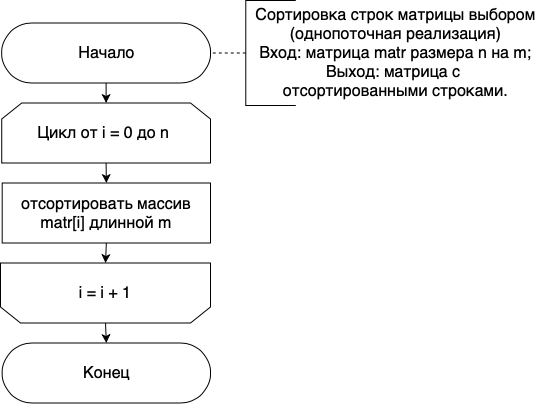
\includegraphics[scale=0.7]{img/select_sort_one_thread_scheme.png}
	\caption{Схема однопоточной реализации сортировки строк матроицы}
	\label{fig:select_sort_one_thread}
\end{figure}

\clearpage

\begin{figure}[h]
	\centering
	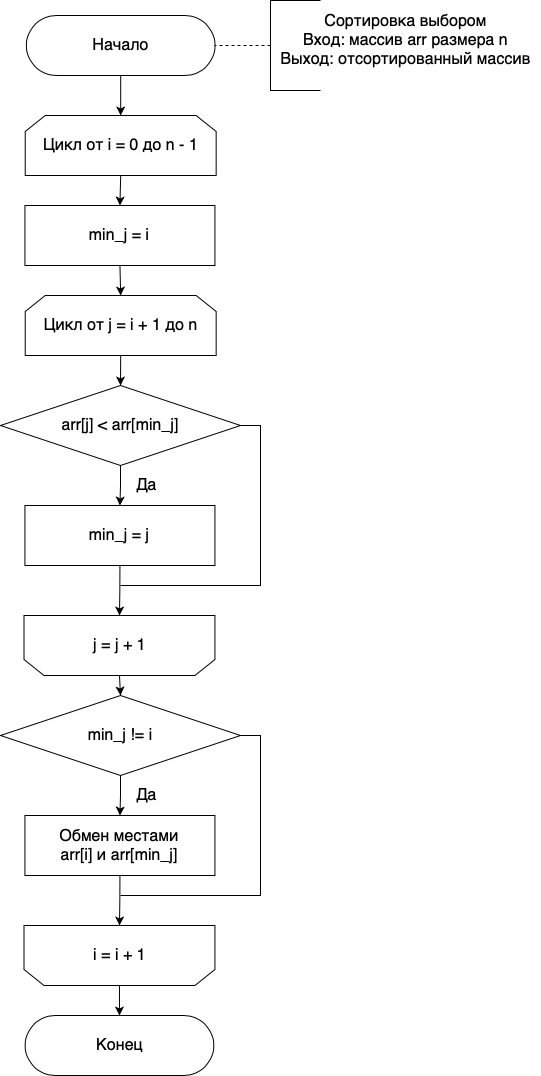
\includegraphics[scale=0.65]{img/select_sort_scheme.png}
	\caption{Схема сортировки массива выбором}
	\label{fig:select_sort}
\end{figure}

\clearpage

\begin{figure}[h]
	\centering
	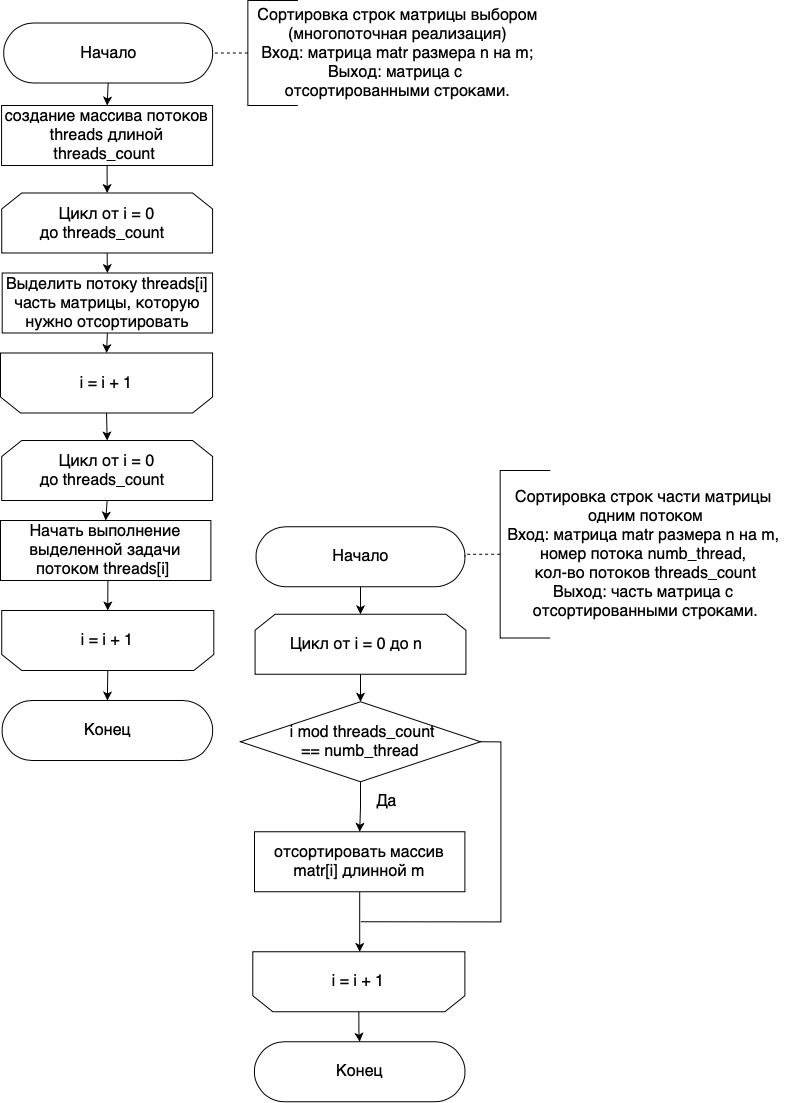
\includegraphics[scale=0.6]{img/select_sort_many_threads_scheme.png}
	\caption{Схема многопоточной реализации сортировки строк матроицы}
	\label{fig:select_sort_many_threads}
\end{figure} 

\clearpage

\section{Классы эквивалентности}

Выделенные классы эквивалентности для тестирования:

\begin{itemize}
	\item кол-во строк матрицы <= 0;
	\item кол-во столбцов матрицы <= 0;
	\item кол-во строк матрицы не является целым числом;
	\item кол-во столбцов матрицы не является целым числом;
	\item кол-во строк и столбцов матрицы равно 1;
	\item строка матрицы содержит одинаковые числа;
	\item все числа в строке матрицы уже отсортированны;
	\item все числа в строке матрицы отсортированны в обратном порядке;
	\item кол-во строк матрицы кратно кол-ву потоков;
	\item кол-во строк матрицы некратно кол-ву потоков.
\end{itemize}

\section{Описание используемых типов данных}

При реализации алгоритмов будут использованы следующие структуры данных:

\begin{itemize}
	\item кол-во строк в матрице - целое число типа $int$;
	\item кол-во столбцов в матрице - целое число типа $int$;
	\item матрица - двумерный массив типа $int$.
\end{itemize}

\clearpage

\section{Структура ПО}

ПО будет состоять из следующих модулей:

\begin{itemize}
	\item $main.cpp$ - файл, содержащий функцию $main$;
    \item $matrix.cpp$ - файл, содержащий функции для работы с матрицами;
    \item $compare.cpp$ - файл, в котором содержатся функции для замера времени работы алгоритмов;
    \item $read.cpp$ - файл, в котором содержатся функции ввода данных;
    \item $sort.cpp$ - файл, в котором содержатся функции для сортировки строк матрицы (с однопоточной и многопоточной реализациями);
    \item $alloc\_free\_memory.cpp$ - файл, в котором содержатся функции для выделения и очищения памяти;
    \item $errors.h$ - файл, в котором содержатся классы для всех ошибок, которые могут возникнуть во время работы программы;
    \item $color.h$ - файл, который содержит макросы для цветного вывода результата работы программы в консоль.
\end{itemize}

Каждый файл с расширением $.cpp$ имеет вспомогательный файл с расширением $.hpp$, где содержатся объявления функций, инклуды и дефайны.

\section{Вывод}

В данном разделе на основе теоретических данных были построены схемы требуемых алгоритмов сортировки строк матрицы, выбраны используемые типы данных, выделены классы эквивалентности для тестирования, а также была описана структура ПО.

\clearpage





\chapter{Технологическая часть}

В данном разделе будут приведены требования к программному обеспечению, средства реализации, листинги кода, а также функциональные тесты.

\section{Требования к программному обеспечению}

\begin{itemize}
    \item входные данные - кол-во строк и столбцов матрицы $matr$ должно быть > 0, все элементы матрицы имеют тип $int$;
    \item выходные данные - матрица $matr$ с отсортированными по возрастанию строками.
\end{itemize}

\section{Средства реализации}

В данной работе для реализации был выбран язык программирования \textit{C++} [2]. Выбор обсуловлен наличием опыта работы с ним. Время работы было замерено с помощью функции \textit{std::chrono::system\_clock::now()} [3].

\clearpage

\section{Листинги кода}

В листингах \ref{lst:select_sort} - \ref{lst:sort_part_matrix} представлены схемы рассматриваемых алгоритмов сортировки строк матрицы.

\begin{center}
\captionsetup{justification=raggedright,singlelinecheck=off}
\begin{lstlisting}[label=lst:select_sort,caption=Функция алгоритма сортировки массива вставками по возрастанию]
void select_sort(int *arr, int n)
{
	int min_j, tmp;
	
	for (int i = 0; i < n - 1; i++)
	{
		min_j = i;

		for (int j = i + 1; j < n; j++)
		{
			if (arr[j] < arr[min_j])
			{
				min_j = j;
			}
		}

		if (min_j != i)
		{
			tmp = arr[i];
			arr[i] = arr[min_j];
			arr[min_j] = tmp;
		}
	}
}
\end{lstlisting}
\end{center}

\clearpage

\begin{center}
\captionsetup{justification=raggedright,singlelinecheck=off}
\begin{lstlisting}[label=lst:select_sort_one_thread,caption=Функция однопоточной реализации сортировки выбором строк матрицы]
void select_sort_one_thread(matrix_h &matr)
{
	for (int i = 0; i < matr.n; i++)
	{
		select_sort(matr.matrix[i], matr.m);
	}
}
\end{lstlisting}
\end{center}

\begin{center}
\captionsetup{justification=raggedright,singlelinecheck=off}
\begin{lstlisting}[label=lst:select_sort_many_threads,caption=Функция многопоточной реализации сортировки выбором строк матрицы]
void select_sort_many_threads(matrix_h &matr, int threads_count)
{   
	std::vector<std::thread> threads(threads_count);

	for (int i = 0; i < threads_count; i++)
	{
		threads[i] = std::thread(sort_part_matrix, std::ref(matr), i, threads_count);
	}

	for (int i = 0; i < threads_count; i++)
	{
		threads[i].join();
	}
}
\end{lstlisting}
\end{center}

\begin{center}
\captionsetup{justification=raggedright,singlelinecheck=off}
\begin{lstlisting}[label=lst:sort_part_matrix,caption=Функция сортировки строк части матрицы для отдельного потока]
void sort_part_matrix(matrix_h &matr, int numb_thread, int threads_count)
{
	for (int i = 0; i < matr.n; i++)
	{   
		if (i % threads_count == numb_thread)
			select_sort(matr.matrix[i], matr.m);
	}
}
\end{lstlisting}
\end{center}

\clearpage

\section{Функциональные тесты}

В таблице \ref{tbl:functional_test} приведены функциональные тесты для однопоточной и многопоточной реализаций сортировки выбором строк матрицы. Все тесты пройдены успешно.

\begin{table}[h]
	\begin{center}
	\begin{threeparttable}
		\captionsetup{justification=raggedright,singlelinecheck=off}
		\caption{\label{tbl:functional_test} Функциональные тесты}
		\begin{tabular}{|c|c|c|c|}
			\hline
			Кол-во строк & Кол-во столбцов & Сама матрица & Ожидаемый результат 
			\\ \hline
			0 & 1 &  & Сообщение об ошибке 
			\\ \hline
			1 & -1 &  & Сообщение об ошибке    
			\\ \hline
			k & 6 &  & Сообщение об ошибке    
			\\ \hline
			1 & 1 &  
			$\begin{pmatrix}
				5
			 \end{pmatrix}$ &
			 $\begin{pmatrix}
				5
			 \end{pmatrix}$      
			\\ \hline
			1 & 3 &  
			$\begin{pmatrix}
				8 $ 8 $ 8
			 \end{pmatrix}$ &
			 $\begin{pmatrix}
				8 $ 8 $ 8
			 \end{pmatrix}$       
			\\ \hline
			1 & 5 &  
			$\begin{pmatrix}
				1 $ 2 $ 3 $ 4 $ 5
			 \end{pmatrix}$ &
			 $\begin{pmatrix}
				1 $ 2 $ 3 $ 4 $ 5
			 \end{pmatrix}$       
			\\ \hline
			1 & 5 &  
			$\begin{pmatrix}
				5 $ 4 $ 3 $ 2 $ 1
			 \end{pmatrix}$ &
			 $\begin{pmatrix}
				1 $ 2 $ 3 $ 4 $ 5
			 \end{pmatrix}$                  
			\\ \hline
			4 & 5 &  
			$\begin{pmatrix}
				17 $ 97 $ 11 $ 52 $ 46 \\
				23 $ 18 $ 81 $ 34 $ 50 \\
				78 $ 78 $ 44 $ 18 $ 20 \\
				61 $ 98 $ 10 $ 12 $ 91 \\
			 \end{pmatrix}$ &
			 $\begin{pmatrix}
				11 $ 17 $ 46 $ 52 $ 97 \\
				18 $ 23 $ 34 $ 50 $ 81 \\
				18 $ 20 $ 44 $ 78 $ 78 \\
				10 $ 12 $ 61 $ 91 $ 98 \\
			 \end{pmatrix}$                   
			\\ \hline
			5 & 3 &  
			$\begin{pmatrix}
				17 $ 97 $ 11 \\
				23 $ 18 $ 81 \\
				78 $ 78 $ 44 \\
				61 $ 98 $ 10 \\
				11 $ 33 $ 22 \\
			 \end{pmatrix}$ &
			 $\begin{pmatrix}
				11 $ 17 $ 97 \\
				18 $ 23 $ 81 \\
				44 $ 78 $ 78 \\
				10 $ 61 $ 98 \\
				11 $ 22 $ 33 \\
			 \end{pmatrix}$              
			\\ \hline
		\end{tabular}
	\end{threeparttable}
	\end{center}
\end{table}

\section{Вывод}

В данном разделе были разработаны алгоритмы для однопоточной и многопоточной реализаций сортировки выбором строк матрицы, проведено тестирование, описаны средства реализации и требования к ПО.





\chapter{Исследовательская часть}

\section{Технические характеристики}

Технические характеристики устройства, на котором выполнялось тестирование представлены далее.

\begin{itemize}
    \item Операционная система: macOS 11.5.2. [4]
    \item Память: 8 GiB.
    \item Процессор: 2,3 GHz 4‑ядерный процессор Intel Core i5. [5]
\end{itemize}

При тестировании ноутбук был включен в сеть электропитания. Во время тестирования ноутбук был нагружен только встроенными приложениями окружения, а также системой тестирования.

\clearpage

\section{Демонстрация работы программы}

\img{220mm}{example}{Пример работы программы}

\clearpage

\section{Время выполнения алгоритмов}

Результаты замеров времени работы однопоточной и многопоточной реализаций алгоритма сортировки выбором строк матрицы приведены на рисунках 4.1 - 4.2. Замеры времени проводились в секундах и усреднялись для каждого набора одинаковых экспериментов.

\begin{table}[h]
	\begin{center}
	\begin{threeparttable}
		\captionsetup{justification=raggedright,singlelinecheck=off}
		\caption{\label{tbl:different_threads} Зависимость времени работы алгоритмов от кол-ва потоков}
		\begin{tabular}{|c|c|c|c|}
			\hline 
			& \multicolumn{3}{c|}{Время работы для матрицы NxM} \\ \cline{2-4}
			Кол-во потоков & 100х100 & 150х150 & 200х200 \\
			\hline
			1 & 0.001472 & 0.004008 & 0.008690 \\
			\hline
			2 & 0.000770 & 0.002127 & 0.004595 \\
			\hline
			4 & 0.000488 & 0.001503 & 0.002507 \\
			\hline
			8 & 0.000445 & 0.001324 & 0.002071 \\
			\hline
			16 & 0.000488 & 0.001144 & 0.002152 \\
			\hline
			32 & 0.000672 & 0.001240 & 0.002262 \\
			\hline
		\end{tabular}
	\end{threeparttable}
	\end{center}
\end{table}

\img{108mm}{graph_different_threads}{Зависимость времени работы алгоритмов от кол-ва потоков (размер матрицы 200х200)}

\clearpage

\begin{table}[h]
	\begin{center}
	\begin{threeparttable}
		\captionsetup{justification=raggedright,singlelinecheck=off}
		\caption{\label{tbl:graph_different_sizes} Зависимость времени работы алгоритмов от размера матрицы (в многопоточной реализации используется 8 потоков)}
		\begin{tabular}{|c|c|c|}
			\hline 
			& \multicolumn{2}{c|}{Время для типа реализации} \\ \cline{2-3}
			Размер матрицы & Однопоточного & Многопоточного \\
			\hline
			100х100 & 0.001472 & 0.000445 \\
			\hline
			110х110 & 0.001822 & 0.000552 \\
			\hline
			120х120 & 0.002237 & 0.000755 \\
			\hline
			130х130 & 0.002762 & 0.000937 \\
			\hline
			140х140 & 0.003358 & 0.001029 \\
			\hline
			150х150 & 0.004008 & 0.001324 \\
			\hline
			160х160 & 0.004776 & 0.001319 \\
			\hline
			170х170 & 0.005545 & 0.001393 \\
			\hline
			180х180 & 0.006478 & 0.001912 \\
			\hline
			190х190 & 0.007525 & 0.001833 \\
			\hline
			200х200 & 0.008690 & 0.002071 \\
			\hline
		\end{tabular}
	\end{threeparttable}
	\end{center}
\end{table}

\img{110mm}{graph_different_sizes}{Зависимость времени работы алгоритмов от размера матрицы (в многопоточной реализации используется 8 потоков)}

\clearpage

\section{Вывод}

В этом разделе были указаны технические характеристики машины, на которой происходило сравнение времени работы однопоточной и многопоточной реализаций алгоритма сортировки выбором строк матрицы.

Многопоточная реализация алгоритма лучше всего работает на 8 потоках. Это связано с тем, что машина, на которой проводилось тестирование, имеет 8 логических ядер. При размере матрицы 200х200 8-ми поточная реализация работает на 17.4\% быстрее 4-х поточной и на 3.8\% быстрее 16-ти поточной. При размере матрицы 100х100 многопоточная реализация (8 потоков) работает на 230.1\% быстрее однопоточной, а при размере 200х200 уже на 319.6\% быстрее.



 

\chapter*{Заключение}
\addcontentsline{toc}{chapter}{Заключение}

Было экспериментально подтверждено различие во временной эффективности однопоточной и многопоточной реализаций сортировки выбором строк матрицы. В результате исследований можно сделать вывод о том, что многопоточная реализация лучше всего работает на 8 потоках, так как машина, на которой проводилось тестирование, имеет 8 логических ядер. Так, например, на матрице размером 200х200 многопоточня (8 потоков) реализация работает на 320\% быстрее однопоточной.

\vspace{5mm}

В ходе выполнения данной лабораторной работы были решены следующие задачи:
\begin{itemize}
	\item изучены основы параллельных вычислений;
	\item применены изученные основы для реализации многопоточного алгоритма сортировки строк матрицы;
	\item экспериментально подтверждено различие во временнoй эффективности однопоточной и многопоточной реализаций алгоритмов при помощи разработанного программного обеспечения на материале замеров процессорного времени;
	\item описаны и обоснованы полученные результаты в отчете о выполненной лабораторной работе, выполненного как расчётно-пояснительная записка к работе.
\end{itemize}

Поставленная цель была достигнута.





\begin{thebibliography}{5}
	\bibitem{bib1}
	Сортировка выбором  [Электронный ресурс]. Режим доступа: \url{https://kvodo.ru/sortirovka-vyiborom-2.html} (дата обращения: 14.10.2021).
	\bibitem{bib2}
	C++ –– Типизированный язык программирования / Хабр[Электронный ресурс]. Режим доступа: \url{https://habr.com/ru/hub/cpp/} (дата обращения: 20.10.2021).
	\bibitem{bib3}
	std::chrono::system\_clock::now - cppreference.com [Электронный ресурс]. Режим доступа: \url{https://en.cppreference.com/w/cpp/chrono/system_clock/now} (дата обращения: 20.10.2021).
	\bibitem{bib4}
	macOS Monterey - Apple(RU) [Электронный ресурс]. Режим доступа: \url{https://www.apple.com/ru/macos/monterey/} (дата обращения: 14.10.2021).
	\bibitem{bib5}
	Intel [Электронный ресурс]. Режим доступа: \url{https://www.intel.ru/content/www/ru/ru/products/details/processors/core/i5.html} (дата обращения: 14.10.2021).
\end{thebibliography}

\addcontentsline{toc}{chapter}{Список литература}

\end{document}
